\documentclass[letterpaper,11pt]{article}
\usepackage{graphicx}
\graphicspath{ {images/} }
\usepackage{wrapfig}
\usepackage{lipsum}
\newlength{\outerbordwidth}
\pagestyle{empty}
\raggedbottom
\raggedright
\usepackage[svgnames]{xcolor}
\usepackage{framed}
\usepackage{tocloft}
\usepackage{amsmath}
\usepackage{etoolbox}
\robustify\cftdotfill

%-----------------------------------------------------------
%Edit these values as you see fit
\setlength{\outerbordwidth}{3pt}  % Width of border outside of title bars
\definecolor{shadecolor}{gray}{0.75}  % Outer background color of title bars (0 = black, 1 = white)
\definecolor{shadecolorB}{gray}{0.93}  % Inner background color of title bars

%-----------------------------------------------------------
%Margin setup
\setlength{\evensidemargin}{-0.25in}
\setlength{\headheight}{-0.25in}
\setlength{\headsep}{0in}
\setlength{\oddsidemargin}{-0.25in}
\setlength{\paperheight}{11in}
\setlength{\paperwidth}{8.5in}
\setlength{\tabcolsep}{0in}
\setlength{\textheight}{9.75in}
\setlength{\textwidth}{7in}
\setlength{\topmargin}{-0.3in}
\setlength{\topskip}{0in}
\setlength{\voffset}{0.1in}

%-----------------------------------------------------------
%Custom commands
\newcommand{\resitem}[1]{\item #1 \vspace{-2pt}}
\newcommand{\resheading}[1]{\vspace{8pt}
  \parbox{\textwidth}{\setlength{\FrameSep}{\outerbordwidth}
    \begin{shaded}

\setlength{\fboxsep}{0pt}\framebox[\textwidth][l]{\setlength{\fboxsep}{4pt}\fcolorbox{shadecolorB}{shadecolorB}{\textbf{\sffamily{\mbox{~}\makebox[6.762in][l]{\large #1} \vphantom{p\^{E}}}}}}
    \end{shaded}
  }\vspace{-5pt}
}

\newcommand{\ressubheading}[4]{
\begin{tabular*}{6.5in}{l@{\cftdotfill{\cftsecdotsep}\extracolsep{\fill}}r}
		\textbf{#1} & #2 \\
		\textit{#3} & \textit{#4} \\
\end{tabular*}\vspace{-6pt}}
%--------------------------------------------------------------------------------------
\begin{document}

%---------------------Personal Information--------------------------------
%---------------------Image Inserted---------------------------------------
\begin{wrapfigure}{r}{4.5cm}
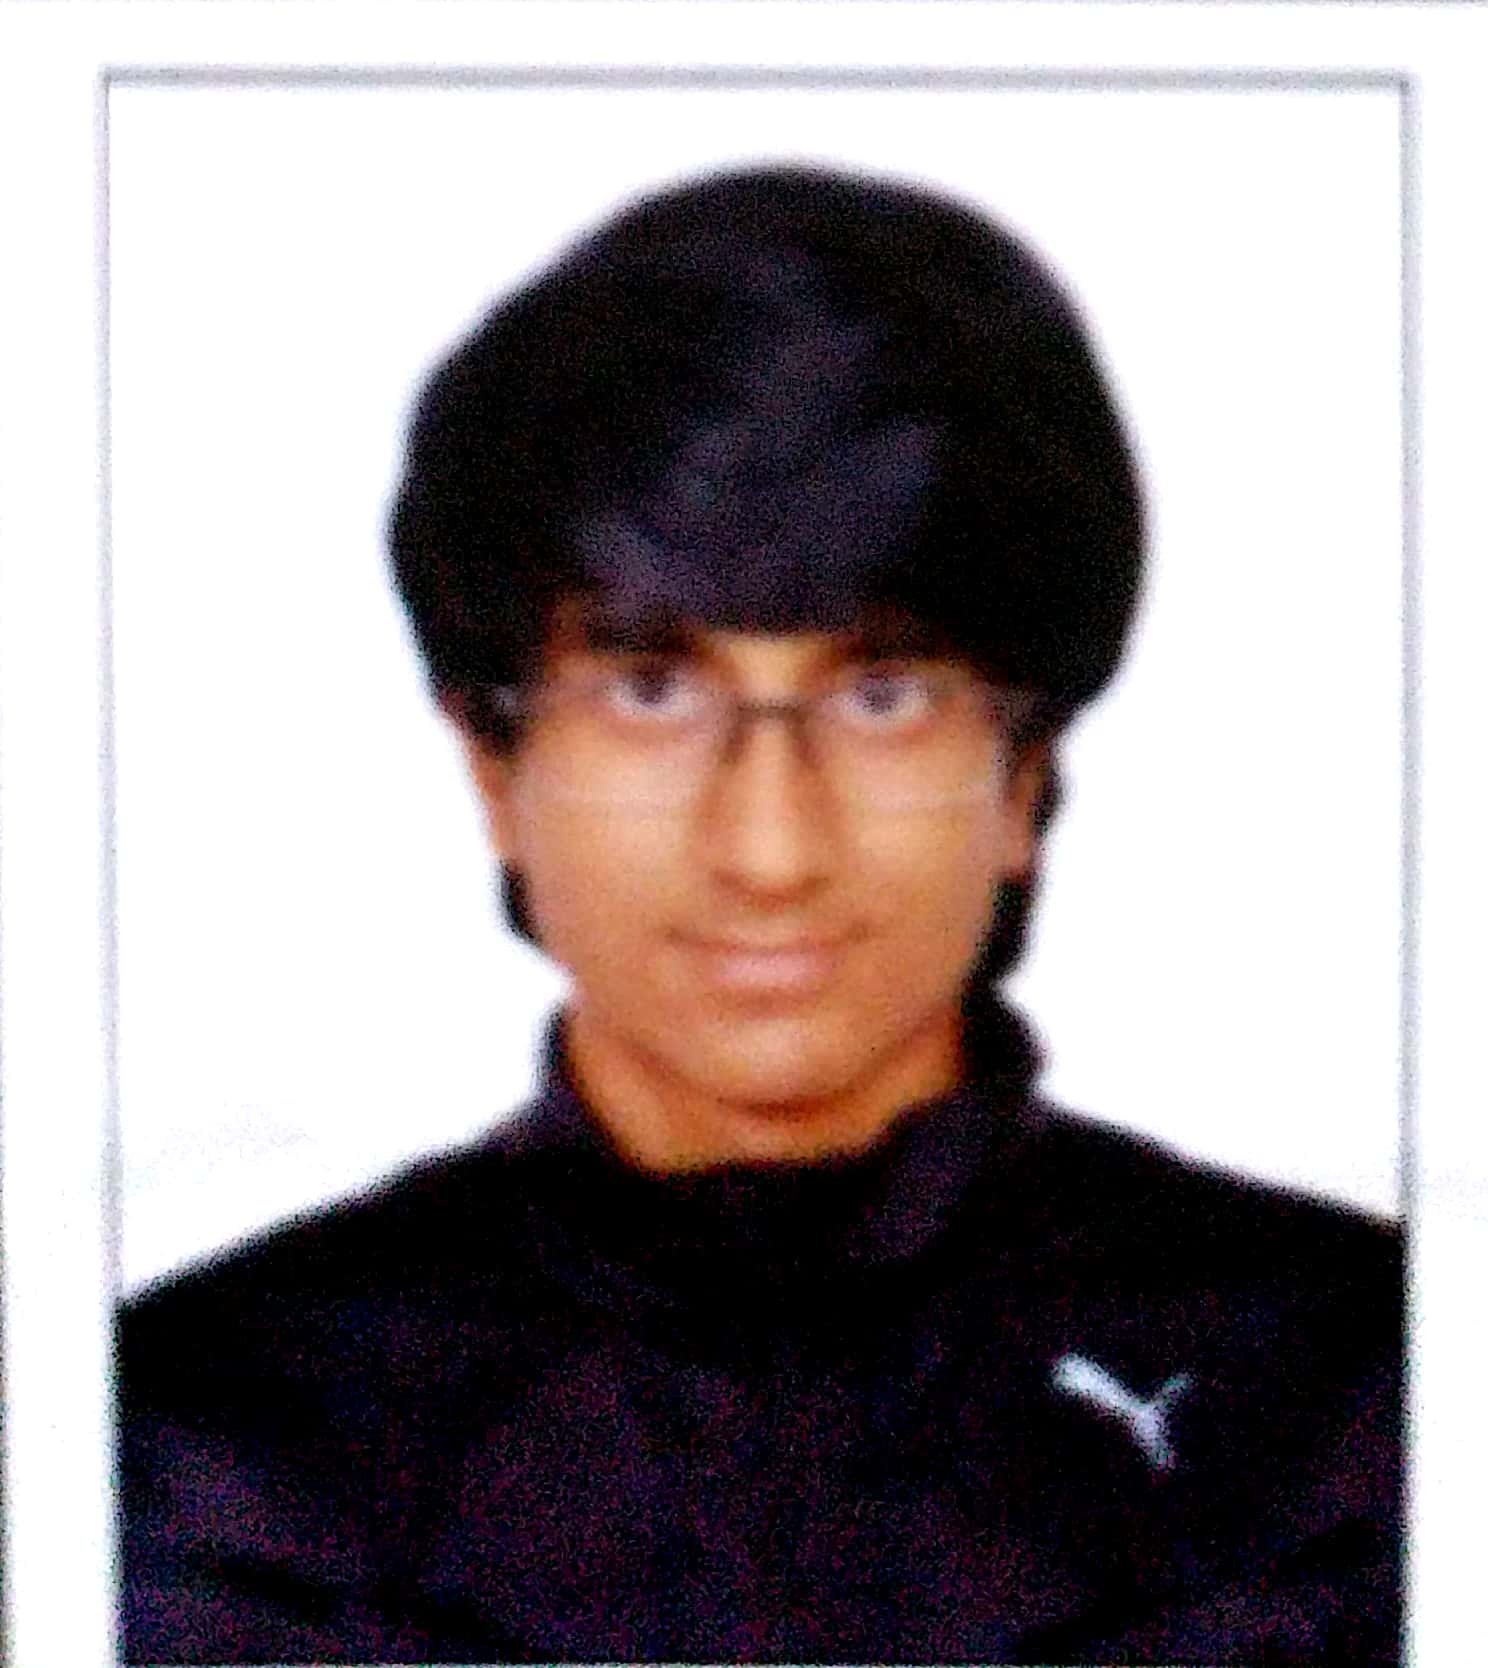
\includegraphics[width=2.5cm]{PHOTO}
\end{wrapfigure} 
%------------------------------------------
\textbf{}  \\
\textbf{{\Large Chirag Shah}}  \\
Email \hspace{0.2cm}  : chirag.ms@somaiya.edu \\
Contact : 9757084146 \\
Address : H-32, 1/2, Panchkamal C.H.S, Sector-29, \\
\hspace{1.8cm}Vashi, Navi Mumbai - 400703 \\ 
%\textbf{}  \\
%------------------------------------------------------------------------------

%----------------------------Career Objective-------------------------------
\resheading{Career Objective}
\textbf{}  \\
Self-Motivated engineering student, trying to develop innovative solutions to simplify tasks through robotics and information technology. Aiming to develop solutions, to improve the efficiency and qualtiy of manual tasks through assistive robotics \\

%-------------------Education--------------------------------------------------
\resheading{Education}

\begin{table}[h!]
  \begin{center}
      \begin{tabular}{l|c|r|l} % <-- Alignments: 1st column left, 2nd middle and 3rd right, with vertical lines in between
      \hspace{0.2cm}\textbf{Year}\hspace{0.2cm} &\hspace{0.2cm} \textbf{Degree/Certificate}\hspace{0.2cm} &\hspace{0.2cm} \textbf{Institute}\hspace{2.3cm} &\hspace{0.2cm} \textbf{CGPA / Percentage}\hspace{0.2cm}\\
      \hline
       2012 & \hspace{0.2cm} Secondary School Certificate \hspace{0.2cm} & \hspace{0.2cm}Fr. Agnel School\hspace{1.7cm} & \hspace{1.2cm} 95.09\% \hspace{0.2cm}\\
       2014 & \hspace{0.2cm} Higher Secondary School Certificate \hspace{0.2cm} & \hspace{0.2cm}Fr. Agnel School\hspace{1.7cm} & \hspace{1.2cm} 86.08\% \hspace{0.2cm}\\
      2014 & \hspace{0.2cm} 1st Semester Btech EXTC \hspace{0.2cm} & \hspace{0.2cm}K.J. Somaiya College of Engineering\hspace{0.2cm} & \hspace{1.2cm} 7.65 \hspace{0.2cm}\\
		2015 & \hspace{0.2cm} 2nd Semester Btech EXTC \hspace{0.2cm} & \hspace{0.2cm}K.J. Somaiya College of Engineering\hspace{0.2cm} & \hspace{1.2cm} 8.54 \hspace{0.2cm}\\
		2015 & \hspace{0.2cm} 3rd Semester Btech EXTC \hspace{0.2cm} & \hspace{0.2cm}K.J. Somaiya College of Engineering\hspace{0.2cm} & \hspace{1.2cm} 8.17 \hspace{0.2cm}\\
		2016 & \hspace{0.2cm} 4th Semester Btech EXTC \hspace{0.2cm} & \hspace{0.2cm}K.J. Somaiya College of Engineering\hspace{0.2cm} & \hspace{1.2cm} 8.8 \hspace{0.2cm}\\
		2016 & \hspace{0.2cm} 5th Semester Btech EXTC \hspace{0.2cm} & \hspace{0.2cm}K.J. Somaiya College of Engineering\hspace{0.2cm} & \hspace{1.2cm} 8.24 \hspace{0.2cm}\\
		2017 & \hspace{0.2cm} 6th Semester Btech EXTC \hspace{0.2cm} & \hspace{0.2cm}K.J. Somaiya College of Engineering\hspace{0.2cm} & \hspace{1.2cm} 8.32 \hspace{0.2cm}\\
		2017 & \hspace{0.2cm} 7th Semester Btech EXTC \hspace{0.2cm} & \hspace{0.2cm}K.J. Somaiya College of Engineering\hspace{0.2cm} & \hspace{1.2cm} 9.32 \hspace{0.2cm}\\
		      
          \end{tabular}
  \end{center}
\end{table}

EXTC - Electronics annd Telecommunication \\

%--------------------------Projects----------------------------------------------------------------
\resheading{Projects}
\textbf{}  \\
\textbf{Autonomous Water Rover} (July 2017 - Present): \\
An autonomous lake monitoring system is being developed, which can also be used for other applications such as depth mapping, fish finding etc. \\
\textbf{}  \\
\textbf{Robo-Rehab} (December 2017 - Present): \\
A continuous passive motion device for the arm, is being developed to aid physiotherapists in rehabilitation of paralysis victims.
\textbf{}  \\
\textbf{}  \\
\textbf{Anomaly Detection in a Bottling Plant} (December 2017 - March 2018): \\
A computer vision based system was designed to detect anomalies such as under filling, over filling in a bottling plant.
\textbf{}  \\
\textbf{}  \\
\textbf{SONAR using ultrasound sensor and Matlab} (March 2016): \\
An ultrasound sensor mounted on a servo was used to get obstacles in a 180 degree field of vision and the results were plotted using matlab.
\textbf{}  \\
\textbf{}  \\
\textbf{Robocon} (November 2015 - March 2016)\\
\textbf{Robocon} (November 2016 - March 2017)


\textbf{}  \\
\end{document}

